
\subsection{Selector Comparison}
\label{sec:selection}

Table~\ref{tab:ladder} reports every rule under identical leave-one-context-out
evaluation, in which the model, its scales, the fixed-policy baseline, the
conformal quantiles and the support envelope are all refitted from the 647
training contexts of each fold, and all five replications of the held-out context
move together. Two findings matter more than the ordering itself.

\begin{table}[htbp]
\centering\footnotesize
\caption{Selector ladder under leave-one-context-out evaluation on 648 contexts.
Regret is in seconds per vehicle. ``Gap closed'' is $G(\pi)$ of
Eq.~\eqref{eq:headroom}: the share of the fixed policy's headroom recovered.
``Top-1'' is the fraction of contexts in which the chosen policy is the observed
best, and is reported to be contrasted with regret, not to rank the rules.}
\label{tab:ladder}
\setlength{\tabcolsep}{3.0pt}
\begin{tabular}{@{}llrrrrrr@{}}
\toprule
& Rule & Mean & Median & Max & CVaR$_{90}$ & Top-1 & Gap closed\\
\midrule
B1 & mechanistic rule & 0.773 & 0.000 & 17.19 & 6.47 & 66.7\,\% & $-71.4$\,\%\\
B0 & fixed policy (SBS) & 0.451 & 0.000 & 17.19 & 3.67 & 64.5\,\% & 0.0\,\%\\
B5 & selective (gated B4) & 0.451 & 0.000 & 17.19 & 3.67 & 64.5\,\% & 0.0\,\%\\
B2 & tree, depth 3 & 0.343 & 0.000 & 17.19 & 3.02 & 73.9\,\% & $+23.8$\,\%\\
B3 & logistic & 0.282 & 0.000 & 17.19 & 2.55 & \textbf{76.1}\,\% & $+37.4$\,\%\\
B4 & advantage GBDT & \textbf{0.199} & 0.000 & \textbf{6.96} & \textbf{1.66} & 73.1\,\% & $\mathbf{+55.8}$\,\%\\
\midrule
& hindsight best (VBS) & 0.000 & 0.000 & 0.00 & 0.00 & 100\,\% & $+100$\,\%\\
\bottomrule
\end{tabular}
\end{table}

\paragraph{The mechanistic rule is more accurate and more expensive than doing
nothing.} B1 identifies the winning policy in 66.7\,\% of contexts against the
fixed policy's 64.5\,\%, and yet its mean regret is 0.773\,s against 0.451\,s ---
it closes $-71$\,\% of the headroom, which is to say it opens a gap of its own.
The explanation is visible in the tail: B1 and B0 share the same worst case, but
B1's CVaR$_{90}$ is 6.47\,s against 3.67\,s. The rule deviates from the fixed
policy in contexts where it is right about the ordering and wrong about the
magnitude, gaining a fraction of a second when correct and losing several seconds
when not. Selecting the right policy more often is not the same as deciding
better, and a study that reported accuracy alone would have concluded that the
mechanistic rule works.

\paragraph{Training on decision cost changes the ordering} B3, the most accurate
rule at 76.1\,\%, is not the cheapest. B4 is less accurate at 73.1\,\% and
recovers substantially more headroom, 55.8\,\% against 37.4\,\%, because it is the
only rule fitted to advantage rather than to the winner's identity: it learns how
much a policy is worth rather than which policy wins, so it deviates from the
fixed policy only where the predicted gain is large. The consequence appears in
the tail statistics, which are the ones an operator would care about. B4 is the
only rule that reduces the worst case, from 17.19\,s to 6.96\,s, and it more than
halves CVaR$_{90}$, from 3.67\,s to 1.66\,s. It deviates from the fixed policy in
233 of 648 contexts and leaves the fixed policy in place in the rest. This is the
predict-then-optimise distinction \citep{elmachtoub2022spo} appearing in a traffic
setting, and it is the one place in this study where the choice of learning target
--- not the choice of model class --- changes the answer.

\paragraph{What the gain is worth} Closing 55.8\,\% of the headroom means
reducing mean journey time from 474.35\,s to 474.10\,s, a saving of 0.25\,s per
vehicle, or 0.053\,\%. The selector works, in the sense that it does what it was
asked to do on held-out contexts, and it is not worth deploying for that gain.
Both halves of that sentence are results.

\subsection{Multi-Criteria Structure}
\label{sec:criteria}

Complementarity looks quite different on the criterion vector than on the scalar.
Over the three criteria jointly, 473 of 648 contexts (73.0\,\%) have more than one
non-dominated policy, and the mean Pareto set contains 2.11 of the four policies
(Fig.~\ref{fig:crit}a). Pareto membership is P3 in 555 contexts, P4 in 525, P2 in
266 and P1 in 21.

The reliability-aware policy is the clearest case of criterion specialisation.
P4 minimises total stopped delay in 429 of 648 contexts, more than any other
policy, while minimising journey time in only 129 and \CO\ in 128
(Fig.~\ref{fig:crit}b). It achieves this by routing to the steady unsignalised
bypass: vehicles spend longer in the network but less of that time stationary.
A study that ranked policies on journey time alone would record P4 as a marginal
member of the portfolio; on stopped delay it is the leading one. The
distance-minimising policy P1 is the opposite case --- it never minimises stopped
delay in any context.

\begin{figure}[htbp]
\centering
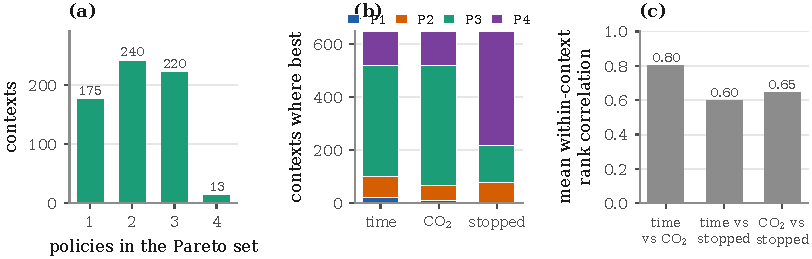
\includegraphics[width=\linewidth]{figures/fig6_criteria.pdf}
\caption{(a) Number of non-dominated policies per context over journey time,
\CO\ and stopped delay. (b) Which policy minimises each criterion, counted over
the 648 contexts. (c) Mean within-context Spearman correlation between criteria
across the four policies, which is the correlation that governs whether the
criteria order policies the same way.}
\label{fig:crit}
\end{figure}

The criteria are correlated but not interchangeable. Pooled across all
context--policy cells the Pearson correlations are 0.94 for journey time against
\CO, 0.89 against stopped delay and 0.89 between \CO\ and stopped delay; but the
quantity that matters for a decision is the within-context correlation across the
four policies, and that is 0.80, 0.60 and 0.65 respectively
(Fig.~\ref{fig:crit}c). The best policy on \CO\ differs from the best on journey
time in 192 contexts (29.6\,\%), and the best on stopped delay differs in 363
(56.0\,\%).

Two consequences follow. First, stopped delay carries decision information that
journey time and \CO\ do not, and it is the criterion on which the portfolio is
most complementary. Second, the close alignment of journey time and \CO\ is the
evidence that led to eco-routing being excluded from the portfolio: with a
within-context rank correlation of 0.80 and identical policy orderings in
52.2\,\% of contexts, a standalone environmental objective has little room to
differ from a time-based one in this network. That exclusion is therefore a
finding about this environment, not an assumption, and it should not be read as a
general statement about eco-routing.

Crucially, a large Pareto set is not evidence that adaptation is valuable. A set
can be large because the criteria disagree about an ordering while all the
differences are small. That is what happens here: 73.0\,\% of contexts have more
than one non-dominated policy, and the decision value on the primary criterion is
0.45\,s per vehicle. Complementarity on the criterion vector and decision value on
the decision criterion are different quantities, and this benchmark separates them
by two orders of magnitude.

\subsection{Distribution Shift}
\label{sec:shift}

Table~\ref{tab:shift} reports the eight splits separately. Pooling them would
produce an average that describes none of them.

\begin{table}[htbp]
\centering\scriptsize
\setlength{\tabcolsep}{3.2pt}
\caption{Distribution shift, by type. Regret is mean decision regret in seconds
per vehicle on the held-out contexts. ``Flagged'' is the share of held-out
contexts the support gate declared outside the training envelope; ``abstained''
is the share on which the selective rule declined to act. A split is classified
as helping or harming when the selector's regret differs from the fixed policy's
by more than the declared 0.05\,s tolerance.}
\label{tab:shift}
\begin{tabular}{@{}llrrrrrrl@{}}
\toprule
Split & Shift type & Tr. & Te. & Fixed & GBDT & Selec. & Flag. & Verdict\\
\midrule
O3 demand $=2400$ & interpolation (control) & 540 & 108 & 0.565 & 0.167 & 0.565 & 0\,\% & helps\\
O2 demand $=1200$ & extrapolation, below & 540 & 108 & 0.528 & 0.531 & 0.528 & 15\,\% & neutral\\
O1 demand $=4200$ & extrapolation, above & 540 & 108 & 0.000 & 0.983 & 0.000 & 43\,\% & \textbf{harms}\\
O4 lag $=300$\,s & extrapolation, above & 432 & 216 & 0.232 & 0.237 & 0.232 & 100\,\% & neutral\\
O5 penetration $=0.8$ & extrapolation, above & 432 & 216 & 0.298 & 0.293 & 0.298 & 100\,\% & neutral\\
O6 green $=0.65$ & extrapolation, above & 432 & 216 & 1.040 & 1.157 & 1.040 & 100\,\% & \textbf{harms}\\
O7 disruption present & covariate $+$ concept & 324 & 324 & 0.630 & 2.216 & 0.630 & 32\,\% & \textbf{harms}\\
O8 north disruption & domain shift & 648 & 54 & 0.314 & 0.176 & 0.314 & \textbf{0\,\%} & helps\\
\bottomrule
\end{tabular}
\end{table}

At the declared tolerance the unguarded selector \textbf{helps on two} splits
(the interpolation control O3 and the domain shift O8), is
\textbf{indistinguishable on three} (O2, O4, O5) and \textbf{harms on three}
(O1, O6 and, worst, the concept shift O7). It is not the case that the selector
degrades under every shift, and it is not the case that shift is harmless; the
behaviour depends on the shift, which is why the splits are not pooled.

Three observations carry most of the content.

\paragraph{The worst failure is the concept shift} O7 trains without any
disruption and tests under disruption, so both the covariate distribution and the
conditional relationship between context and policy performance change. The fixed
policy incurs 0.630\,s of regret there; the selector incurs 2.216\,s, more than
three times as much. Extrapolating a factor level is survivable in this benchmark;
learning a relationship that no longer holds is not.

\paragraph{Extrapolation above the training range is where the selector does
damage.} O1 holds out the highest demand. There the fixed policy is optimal in
every one of the 108 held-out contexts, so its regret is exactly zero, and any
deviation is pure loss: the selector incurs 0.983\,s. A tree-based regressor
cannot extrapolate --- beyond the largest training value of a feature it returns
the prediction of its outermost leaf --- and here that leaf was fitted where the
fixed policy was not always best.

\paragraph{The support gate does not detect the shift it was built for} The gate
flags 100\,\% of held-out contexts on the three extrapolation splits O4, O5 and
O6, which is the behaviour it was designed for. It flags 43\,\% on O1 and 32\,\%
on O7. It flags \textbf{none} of the 54 held-out contexts of O8
(Fig.~\ref{fig:shift}b), despite O8 being the only genuine domain shift in the
set. The reason is not a tuning failure but a representation failure: the
descriptor $x_7$ encodes that a disruption may occur, not where it occurs, so a
disruption relocated to a different corridor is invisible in the feature space the
gate operates in. A detector that measures distance in a feature space cannot
detect a change that the feature space does not encode. This is a general
limitation of support-based out-of-distribution detection, and it is exactly the
case in which such a gate would be most relied upon. No claim of out-of-
distribution safety is made anywhere in this paper.

\begin{figure}[htbp]
\centering
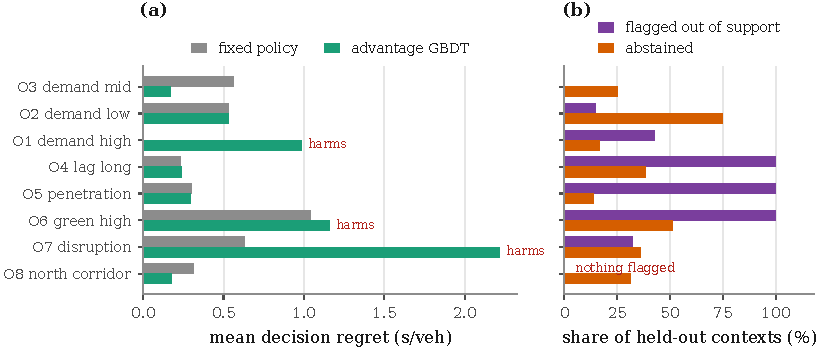
\includegraphics[width=\linewidth]{figures/fig7_shift.pdf}
\caption{(a) Mean decision regret of the fixed policy and the advantage GBDT on
each held-out split. (b) Share of held-out contexts flagged outside the training
support and share on which the selective rule abstained. The support gate flags
every context of the three factor-level extrapolations and none of the domain
shift O8.}
\label{fig:shift}
\end{figure}

\subsection{Selective Prediction}
\label{sec:selective}

The selective rule B5 acts only when the context is inside the support envelope
and the split-conformal lower bound on the predicted advantage is positive.
Its behaviour in this study is unambiguous and entirely negative:

\begin{quote}
B5 chose the fixed policy in \emph{every one} of the 648 contexts, and on
\emph{every one} of the eight shift splits. It abstained in exactly the 233
contexts in which the unguarded selector would have deviated, and in the
remaining 415 the unguarded selector chose the fixed policy anyway. The
confidence gate never certified a single deviation.
\end{quote}

This is not a tuning failure, and it is not a property of the particular
conformal construction. It follows from a ratio. The mean replication noise
floor across contexts --- the largest paired $2\,$SE against the best policy ---
is 20.90\,s per vehicle. The mean advantage available to any deviation is
0.45\,s. A conformal interval calibrated to residuals of that magnitude is
necessarily far wider than the effect it is being asked to certify, so the lower
bound on a predicted advantage is essentially never positive. Any confidence-gated
selector, conformal or otherwise, faces the same arithmetic in this regime.

The consequence is a design rule that generalises beyond this study, and it is
the reverse of the usual framing. Selective prediction is normally presented as
insurance: give up a little in-distribution performance to avoid
out-of-distribution harm. Here the insurance costs everything and pays nothing,
because the premium --- the entire 55.8\,\% of headroom that B4 recovers --- is
larger than the loss being insured against in every split where the selector helps,
and the gate cannot distinguish the splits where it harms. Before building an
abstention mechanism, the effect size should be compared against the replication
noise of the system it will act on; if the ratio is of the order seen here, no
confidence gate can act.

\subsection{Sensitivity and Robustness}
\label{sec:robust}

\paragraph{Policy parameters} Two parameters had to be chosen and were frozen:
the admissibility tolerance $\epsilon$ of P3 and the risk weight $\lambda$ of P4.
Re-simulating a 96-context subset shows that the choice matters, and in one case
matters a great deal. Loosening P3's tolerance from the frozen $\epsilon=0.20$ to
$0.30$ improves its mean journey time by 16.66\,s per vehicle; tightening it to
$0.10$ costs 8.10\,s. Changing P4's $\lambda$ from 1.0 to 0.5 or 1.5 changes its
mean cost by $-0.11$\,s and $+1.27$\,s, with a median change of exactly zero in
both cases, so P4 is insensitive to its parameter over this range while P3 is not.

The frozen values are not revised, and the main analysis is not recomputed at the
better value: doing so after seeing the result would replace a pre-declared
benchmark with a tuned one. The correct reading is that the benchmark is
\emph{conservative} with respect to P3 and that parameter tuning within a single
policy is worth roughly 37 times more on this benchmark than selecting among
policies. That comparison is arguably the most practically useful number in the
study, and it was produced by a robustness check rather than by the main
experiment.

\paragraph{Preference weights} Scoring the three criteria under three declared
normalised profiles changes the preferred policy in 14.5\,\% of contexts. The
time-weighted profile agrees with the primary criterion in 92.9\,\% of contexts,
the balanced profile in 86.0\,\% and the environment-weighted profile in 80.1\,\%.
The decision is therefore not inert with respect to the preference model --- in
contrast to what a strongly aligned criterion set would produce --- but neither is
it dominated by it.

\paragraph{Model capacity} The ladder of Table~\ref{tab:ladder} is itself the
capacity sensitivity: depth-2 tree, depth-3 tree, logistic regression and
gradient boosting span a wide range of flexibility, and the ordering by regret
does not follow the ordering by capacity. The best rule by regret is not the best
by accuracy, and the simplest rule is worse than no rule at all.
